% !TEX root = PREN2_Dokumentation.tex

\section{Projektmanagementplan}\label{Projektmanagementplan}

\subsection{Projektorganisation}
\subsubsection{Organisationsplan, Rollen, Zuständigkeiten}
In nachfolgendem Diagramm sind alle Projektbeteiligten aufgeführt. Die Projektmitglieder von der Hochschule Luzern Technik und Architektur unterstehen dabei in diesem Projekt keiner hier genannten Person. Sie haben aus ihrem Projekt entsprechend eigene Projektorganisationen. 
\begin{figure}[H]
    \centering
    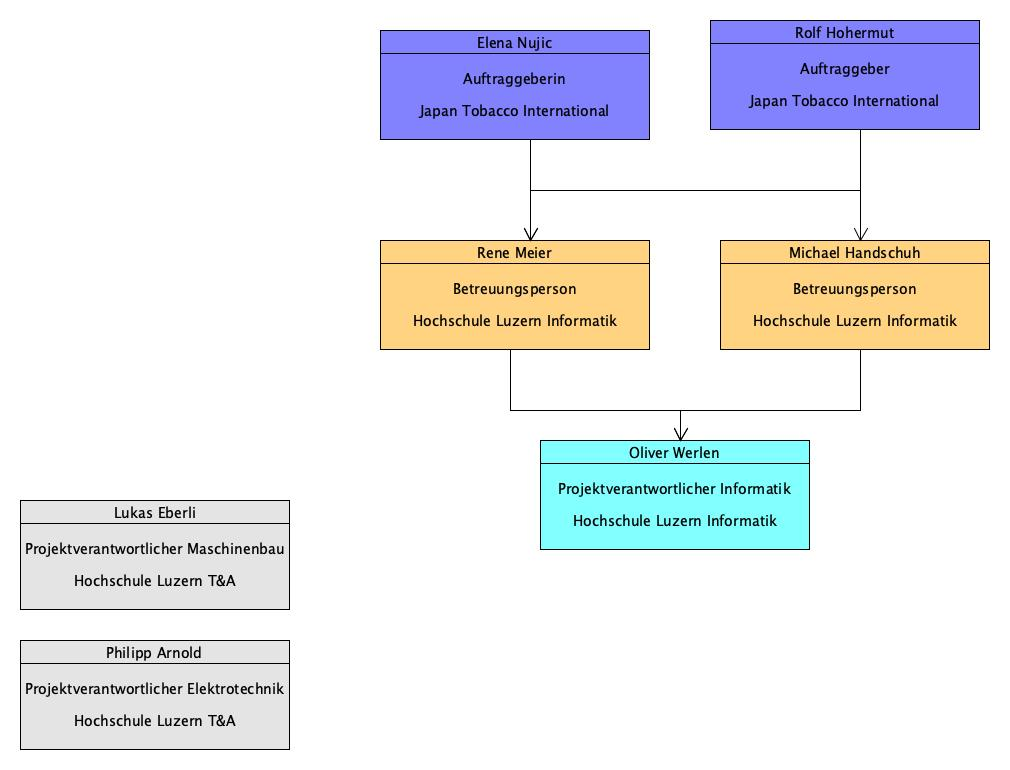
\includegraphics[width=1\textwidth]{images/Organigramm_BAA.jpg}
    \caption[Organigramm]{Organigramm, Quelle: Autor}
    \label{img: OrganigrammWiPro}
\end{figure}	

\paragraph{Rollen}
Im Projekt wird nach dem hybriden Projektmanagementvorgehen \gls{SoDa} gearbeitet. Es werden die hier genutzten Rollen beibehalten. 
\begin{itemize}
	\item Projektleiter/in
	\item Product Owner
	\item Scrum Master
	\item Scrum Team
\end{itemize}
[\cite{sodaHSLU}]
Da es jedoch in diesem Projekt nur einen aktiven Projektmitarbeiter gibt, werden alle Rollen von Oliver Werlen übernommen. 
\subsubsection{Projektstrukturplan}

\begin{figure}[H]
    \centering
    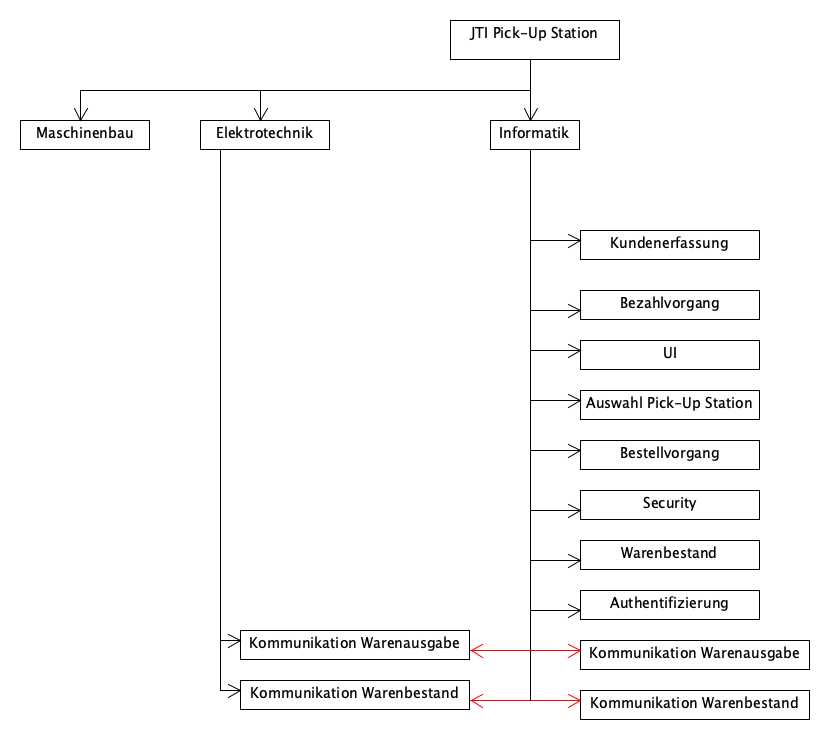
\includegraphics[width=1\textwidth]{images/pmp.png}
    \caption[Projektstrukturplan]{Projektstrukturplan,\\ Quelle: Autor}
    \label{img: Projektstrukturplan}
\end{figure}

\paragraph{Beschreibung}
Im obigen Projektstrukturplan in Abbildung \ref{img: Projektstrukturplan} werden die wichtigsten Teilbereiche der Applikation aufgelistet. Dabei wird der Fokus auf den Informatikteil gelegt. Es werden einzig die Schnittstellen zur Elektrotechnik berücksichtigt. Diese wurden rot eingezeichnet. Die Teilbereiche beziehen sich dabei hauptsächlich auf die in \ref{RSR} erarbeiteten Anforderungen. 
\newpage
\subsection{Projektführung}
\subsubsection{Rahmenplan}

Im untenstehenden Rahmenplan wird mittels Zeitstrahl eine Grobplanung dargestellt. 

\begin{figure}[H]
    \centering
   \includegraphics[width=1\textwidth]{images/SoDa_Zeitstrahl.png}
    \caption[SoDa Rahmenplan]{Rahmenplan,\\ Quelle: Autor}
    \label{img: SoDa Rahmenplan}
\end{figure}
Der Rahmenplan wurde zu Beginn des Projekts grob dargestellt. Im Verlauf des Projekts kann dieser bei Bedarf angepasst werden. Die einzelnen Versionen des Rahmenplans sind im Anhang \ref{Rahmenplaene} zu finden. 
\newpage

\subsubsection{Meilensteine}\label{Meilensteine}
Wie in Abbildung \ref{img: SoDa Rahmenplan} zu sehen gibt es insgesamt sieben Meilensteine.
Diese werden in folgender Tabelle beschrieben sowie die nötigen Deliverables aufgezeigt.


\begin{table}[H]
\setlength\extrarowheight{2pt} % for a bit of visual "breathing space"
\begin{tabularx}{\textwidth}{|C|C|C|}
\hline
\textbf{Meilenstein} &  \textbf{Beschreibung} & \textbf{Deliverables}  \\

\hline
Projektstart & Das Kick-Off Meeting mit allen Projektteilnehmern wurde durchgeführt und das Projekt freigegeben. & Finale Aufgabenstellung\\

\hline
Abschluss Initialisierungsphase & In der Initialisierungsphase wurden alle zum erfolgreichen Start benötigten Unterlagen erstellt. Die Anforderungen wurden von allen Projektmitgliedern akzeptiert. & Projektmanagementplan, Systemspezifikation, Anforderungsliste\\


\hline
Abschluss Bestellprozess & Der Bestellprozess \glqq Artikelauswahl, Artikel in Warenkorb, Artikel Bezahlen\grqq{} sowie die Kundenregistrierung sind umgesetzt und getestet. & Testprotokolle zu Abschluss Bestellprozess, Demo Bestellprozess, Release Bestellprozess 
\newline
\textbf{Release 1}
 \\
 
 \hline
Zwischenpräsentation & Die Zwischenpräsentation ist durchgeführt worden.  & Zwischenpräsentation im Anhang, Sitzungsprotokoll
 \newline
 \\

\hline
Abschluss Realisierungsphase & Die noch fehlenden Anforderungen aus dem vorherigen Meilenstein sind hier abzuliefern. Es handelt sich dabei um die Auswahl sowie die Abholung an einer Pick-Up Station. Zudem ist die Abfrage des Warenbestandes Teil dieses Meilensteins. & Testprotokolle zu Abholung, Testprotokolle Auswahl, Integration alte Daten, Demo verschiedene Features
\newline
\textbf {Release 2}
\\

\hline
Start Einführung & Der Auftraggeber erhält eine Einführung in die Software. & Sitzungsprotokoll zum Ende der Einführungsphase  
\\

\hline
Projektende & Der Auftraggeber erhält eine Einführung in die Software & Fertige Projektdokumentation, Abgeschlossene Testprotokolle   
\newline
\textbf{Release 3}
\\
\hline
Abschlusspräsentation & Die Abschlusspräsentation ist durchgeführt worden.  & - 
\newline
\\
\hline

\end{tabularx}
\caption{ \label{tbl: Meilensteine}Meilensteine, Quelle: Autor}
\end{table}
\newpage
\subsubsection{Risikomanagement}\label{risikomanagement}
Beim Risikomanagement werden die wichtigsten Risiken für das Projekt ermittelt und passende Gegenmassnahmen ausgearbeitet. 

\begin{table}[H]
\setlength\extrarowheight{2pt} % for a bit of visual "breathing space"
\begin{tabularx}{\textwidth}{|C|C|C|}
\hline
\textbf{Risiko} & \textbf{Eintrittswahrsch.} & \textbf{Schaden} \\

\hline
Falsche Zeiteinschätzung &  70 & 80\\
\hline
Requirements nehmen zu / Requirements ändern sich & 60 & 60\\
\hline
Entwicklerausfall & 40 & 70\\
\hline
Unklare Schnittstellenspez. & 40 & 70\\
\hline
Vernachlässigung Designprozess & 20 & 60\\
\hline
Fehlende technische Kompetenz & 20 & 90\\
\hline
Veränderung im Projektteam & 10 & 70\\
\hline
\end{tabularx}
\caption{ \label{tbl: Risikoanalyse}Risikoanalyse, Quelle: Autor}
\end{table}
\begin{figure}[H]
    \centering
    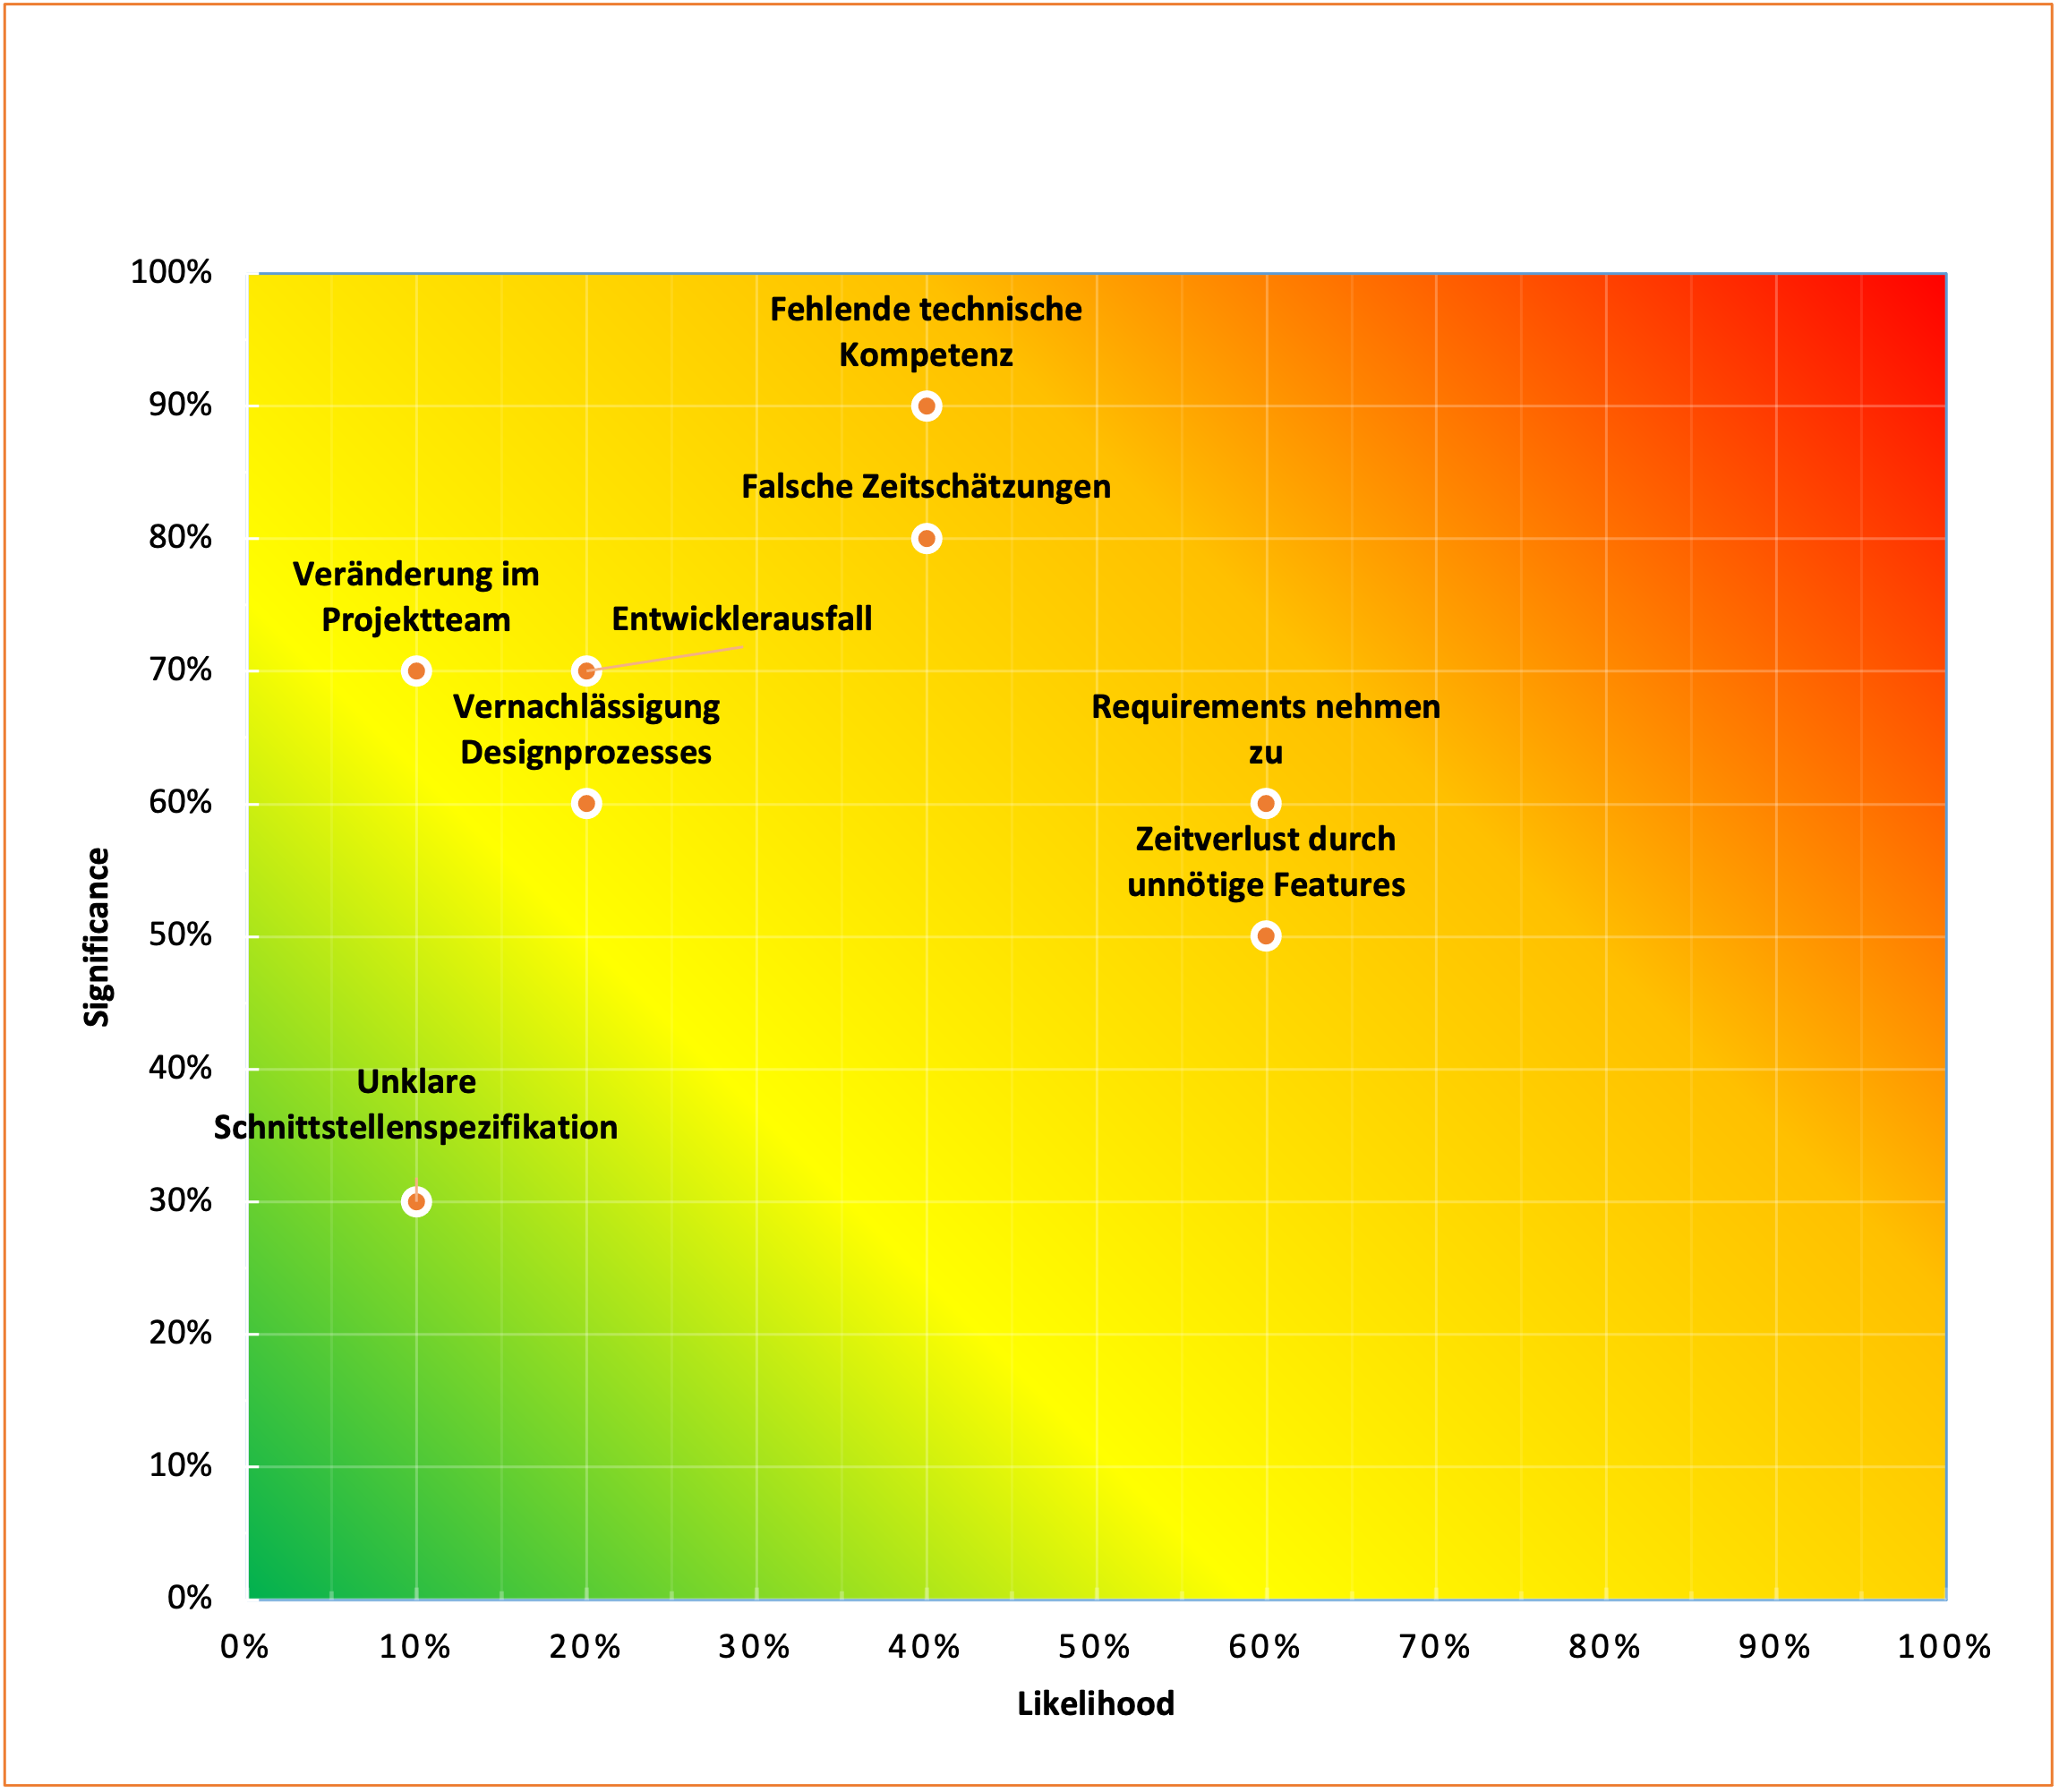
\includegraphics[width=1\textwidth]{images/RiskMap.png}
    \caption[Risikomatrix]{Risikomatrix,\\ Quelle: Autor}
    \label{img: Risikomatrix}
\end{figure}

\paragraph{Beschreibung}
Basierend auf der Risikomatrix in Abbildung \ref{img: Risikomatrix} müssen für die Risiken im rechten oberen Viertel Gegenmassnahmen erarbeitet werden.In diesem Viertel liegt allerdings nur das Risiko "Requirements nehmen zu". Aus diesem Grund werden hier noch weitere Risiken bearbeitet. 
\begin{itemize}
\item Requirements nehmen zu
\item Zeitverlust durch unnötige Features
\item Falsche Zeiteinschätzung
\item Fehlende technische Kompetenz
\end{itemize}

\paragraph{Gegenmassnahmen}
\subparagraph{Requirements nehmen zu}
Um eine Veränderung der Requirements während des Projekt zu vermeiden, werden die Requirements in ständigem Kontakt mit den Auftraggebern erarbeitet und von diesen abgenommen. 
\subparagraph{Zeitverlust durch unnötige Features}
Um dies zu verhindern werden die entsprechenden User Stories definiert. Es werden dabei nur die Requirements berücksichtigt, welche beim Requirements Engineering erarbeitet und vom Auftraggeber abgenommen wurden. 
 \subparagraph{Falsche Zeiteinschätzung}
Um eine bessere Zeiteinschätzung zu erlangen, wird auf das Wissen aus vorherigen Projekten zurückgegriffen. Basierend darauf kann die Planung genauer durchgeführt werden. 
 \subparagraph{Fehlende technische Kompetenz}
Es werden Technologien verwendet, welche bereits bekannt sind. Zudem finden diese in vielen Projekten Anwendung, sodass auf das Wissen von erfahrenen Entwicklern zurückgegriffen werden kann. 

\begin{table}[H]
\begin{tabularx}{\textwidth}{|C|C|C|}
\hline
\textbf{Risiko} & \textbf{Eintrittswahrsch.} & \textbf{Schaden} \\
\hline
Requirements nehmen zu / Requirements ändern sich & 20 & 10\\
\hline
Zeitverlust unnötige Features & 30 & 40\\
\hline
Falsche Zeiteinschätzung &  30 & 80\\
\hline
Fehlende technische Kompetenz & 20 & 20\\
\hline
\end{tabularx}
\caption{ \label{tbl: RisikoanalyseNachMassnahmen}Risikoanalyse nach Massnahmen, Quelle: Autor}
\end{table}

\begin{figure}[H]
    \centering
   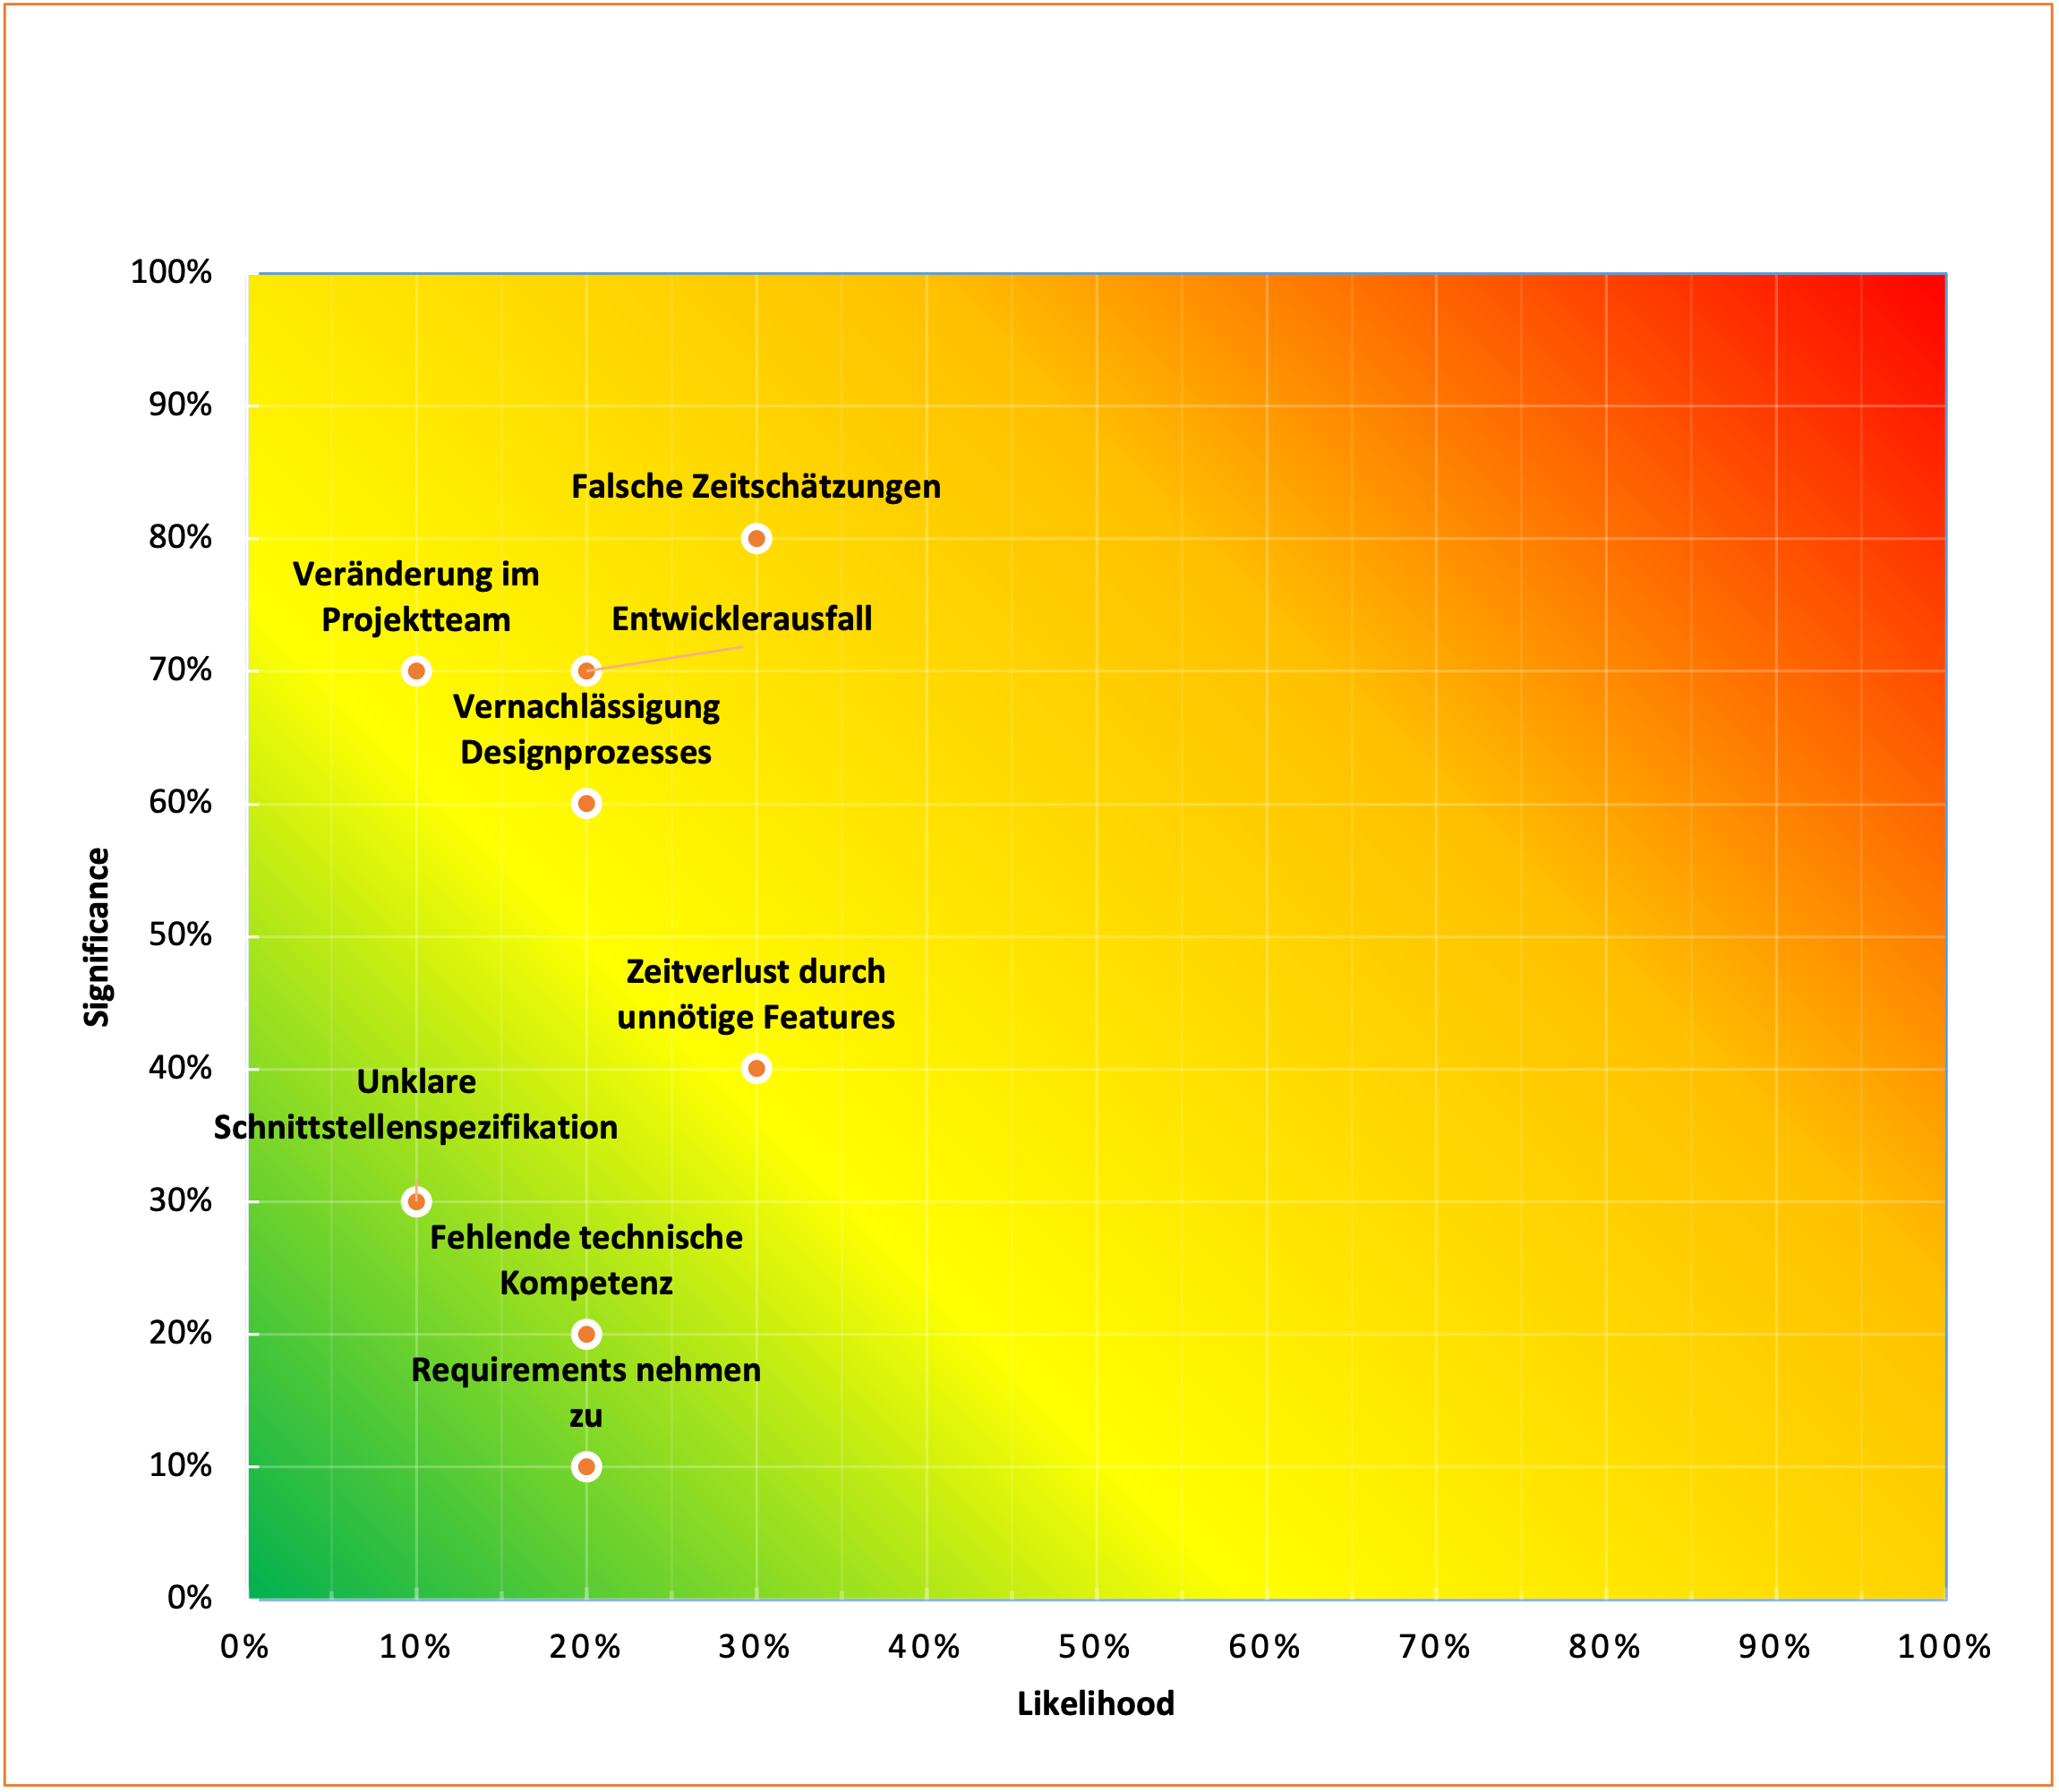
\includegraphics[width=1\textwidth]{images/RiskMap_naher.png}
    \caption[Risikomatrix nach Massnahmen]{Risikomatrix nach Massnahmen,\\ Quelle: Autor}
    \label{img: RisikomatrixNachher}
\end{figure}

\subsubsection{Definition of done}
In jedem Sprint müssen die nachfolgenden Punkte zwingend erreicht werden, um ein potenziell auslieferbares Produkt zu erhalten.

\begin{itemize}
\item Review durchgeführt
\item Akzeptanzkriterien erfüllt
\item keine kritischen Bugs
\item Clean Code Guidelines eingehalten
\item Dokumentation aktuell
\end{itemize}
\newpage
\subsection{Projektunterst\"utzung}
\subsubsection{Tools f\"ur Entwicklung, Test und Abnahme}
\paragraph{Entwicklungstools}
Bei der Entwicklung des Projekts kommen folgende Programme zum Einsatz. 

\begin{table}[H]
\setlength\extrarowheight{2pt} % for a bit of visual "breathing space"
\begin{tabularx}{\textwidth}{|C|C|C|}
\hline
\textbf{Typ} &\textbf{Tool} & \textbf{Version}  \\

\hline
IDE & Intelij Ultimate  & 2020.1\\
\hline
IDE & Visual Studio Code & 1.53.2\\ 
\hline
Versionsverwaltung & Git & 2.27.0\\
\hline
Datenbank & Git & 10.5.10 \\
\hline
Frameworks & Node.js & 14.13.0 \\
\hline
 & Spring Boot & 12.4.3 \\
 \hline
 & Angular & 11 \\
 \hline
Sprachen & TypeScript& 4.3 \\
\hline
& Java& 11 \\
\hline
\end{tabularx}
\caption{ \label{tbl: Entwicklungstools}Entwicklungstools, Quelle: Autor}
\end{table}
\subsubsection{Konfigurationsmanagement}
\paragraph{Konfigurationseinheit}

Bei diesem Projekt besteht eine Konfigurationseinheit aus mehreren Teilen. Dabei werden diese bei jedem Release aufgeführt. Zusätzlich dazu kommen noch die Reports der automatisierten Tests, falls vorhanden auch der Systemtests.
\begin{itemize}
\item Spring Applikation
\item Webapplikation
\item Raspberry Pi Client
\end{itemize}
\paragraph{Release 1}\label{release1}

\begin{table}[H]
\setlength\extrarowheight{2pt} % for a bit of visual "breathing space"
\begin{tabularx}{\textwidth}{|C|C|C|}
\hline
\textbf{Typ} &  \textbf{Version}  \\
\hline
Spring Applikation & 1.0.0 \\
\hline
Webapplikation  & 1.0.0\\
\hline
Raspberry Pi Client  & 0.0.0\\

\hline
\end{tabularx}
\caption{ \label{tbl: Konfigurationseinheit Release 1}Konfigurationseinheit Release 1, Quelle: Autor}
\end{table}

\paragraph{Testprotokolle}
Die gesamten Testprotokolle sind im Anhang \ref{testprotokolleBestellung} zu finden. 
\newpage
\paragraph{Release 2}\label{release2}

\begin{table}[H]
	\setlength\extrarowheight{2pt} % for a bit of visual "breathing space"
	\begin{tabularx}{\textwidth}{|C|C|C|}
		\hline
		\textbf{Typ} &  \textbf{Version}  \\
		\hline
		Spring Applikation & 1.4.6\\
		\hline
		Webapplikation  & 1.1.3\\
		\hline
		Raspberry Pi Client  & 0.1.0\\
		\hline
	\end{tabularx}
	\caption{ \label{tbl: Konfigurationseinheit Release 2}Konfigurationseinheit Release 2, Quelle: Autor}
\end{table}

\paragraph{Testprotokolle}
Die gesamten Testprotokolle sind im Anhang \ref{testprotokolleRealisierungsphase} zu finden. 
\paragraph{Release 3}\label{release3}

\begin{table}[H]
	\setlength\extrarowheight{2pt} % for a bit of visual "breathing space"
	\begin{tabularx}{\textwidth}{|C|C|C|}
		\hline
		\textbf{Typ} &  \textbf{Version}  \\
		\hline
		Spring Applikation & 1.4.7\\
		\hline
		Raspberry Pi Client  & 1.1.0\\
		\hline
	\end{tabularx}
	\caption{ \label{tbl: Konfigurationseinheit Release 3}Konfigurationseinheit Release 3, Quelle: Autor}
\end{table}

\paragraph{Testprotokolle}
Die gesamten Testprotokolle sind im Anhang \ref{testprotokolleRealisierungsphase} zu finden. 
\newpage
\subsection{Teststrategie und Drehbuch}
\subsubsection{Teststrategie}
Es handelt sich hier um die Entwicklung eines Prototypen. Die Priorität wird entsprechend gesetzt. 
\begin{itemize}
	\item Funktionalität vor Design
	\item Sicherheit vor Tempo
	\item Funktionalität vor Testing
\end{itemize}
Aus diesem Grund wurden die Unit- und Integrationtests nur konzeptuell umgesetzt. Bei Bedarf können diese erweitert werden. 

\paragraph{Automated Testing der REST-Schnittstelle}
Zum Testen der \ac{REST}-Schnittstelle wird dabei in erster Linie Postman genutzt. 

\subsubsection{Testdrehbuch}\label{testsvonmeilensteine}
Wie oben genannt wird auf manuelles Testing gesetzt. 
Die Tests gehen mit den gleichnamigen Meilensteinen einher.
Nachfolgend werden diese inklusive den erhaltenen Resultate beschrieben.\\

Die Testdrehbücher sind dabei direkt in die Testprotokolle \ref{Testprotokolle} integriert. An dieser Stelle wird auf ein erneutes Beschreiben verzichtet. 

\subsection{Bemerkungen}
Zur Erstellung des Projektmanagementplans wurde die Vorlage der Hochschule Luzern verwendet. [\cite{pmpHSLU}]
\newpage
